\documentclass[11pt]{easymemo3}

%\SectionNumber
%\BlackAndWhite
\usepackage{lscape}
\usepackage{multirow}

\begin{document}


\MakeTitle{2024.11.5}{調和関数}{明大理工 楠瀬博明}


\section{多極子球面調和関数と表現行列}

本稿の座標はすべてCartesian座標$(x,y,z)$である。

\subsection{定義と性質}

スケールされた球面調和関数(Condon-Shortley位相を採用)
\begin{align}
O_{l,m}(\bm{r})=\sqrt{\frac{4\pi}{2l+1}}r^{l}Y_{l,m}(\hat{\bm{r}}),
\quad
(l=0,1,2,\cdots;\, m=l,l-1,\cdots,-l),
\quad
\hat{\bm{r}}=\frac{\bm{r}}{r},
\quad
r=|\bm{r}|
\end{align}
は連続回転群SO(3)の既約表現である。
この関数は、空間反転操作$\mathcal{P}$ ($\bm{r}\to-\bm{r}$; $\theta\to\pi-\theta$, $\phi\to\phi+\pi$)に対して、$\mathcal{P}[O_{l,m}(\bm{r})]=O_{l,m}(-\bm{r})=(-1)^{l}O_{l,m}(\bm{r})$の性質をもつ極性のスカラー関数である。
すなわち、$O_{l,m}$に対する空間反転操作の表現行列は$(2l+1)\times(2l+1)$の単位行列を$\hat{1}^{(l)}$として
\begin{align}
\mathcal{P}\to(-1)^{l}\hat{1}^{(l)}
\end{align}
である。
また、$[O_{l,m}(\bm{r})]^{*}=(-1)^{m}O_{l,-m}(\bm{r})$が成り立つ。



球面調和関数$O_{l,m}(\bm{r})$と極性の内部自由度$\vec{q}_{s,n}$ ($2s+1$成分のベクトル; $\vec{q}_{s,m}^{\,*}\cdot\vec{q}_{s,n}=\delta_{m,n}$)の合成から多極子球面調和関数(multipolar spherical harmonics)を次のように定義する\footnote{$\vec{q}_{s,n}$の基底$\alpha$による表示は$\braket{\alpha|s,n}=U_{n,\alpha}^{(s)*}$である。}。
\begin{align}
&
\vec{O}_{l,m}^{(s,k)}(\bm{r};\vec{q})=i^{s+k}(-1)^{l+m}\sqrt{2l+1}\sum_{n=-s}^{s}
\begin{pmatrix} l+k & l & s \\ m-n & -m & n \end{pmatrix}O_{l+k,m-n}(\bm{r})\vec{q}_{s,n},
\cr&\quad
(l=0,1,2,\cdots;\,m=l,l-1,\cdots,-l;\,s=0,1,2,\cdots;\,k=-s,-s+1,\cdots,s).
\end{align}
ここで、$[\vec{q}_{s,n}]^{*}=(-1)^{n}\vec{q}_{s,-n}$, $\mathcal{P}[\vec{q}_{s,n}]=(-1)^{s}\vec{q}_{s,n}$である。
$3j$記号の下行の符号をすべて反転させると$(-1)^{l+k+l+s}=(-1)^{k+s}$の因子がかかること等を用いると、以下の関係が示される。
\begin{align}
&
[\vec{O}_{l,m}^{(s,k)}(\bm{r};\vec{q})]^{*}=(-1)^{m}\vec{O}_{l,-m}^{(s,k)}(\bm{r};\vec{q}),
\\&
\mathcal{P}[\vec{O}_{l,m}^{(s,k)}(\bm{r};\vec{q})]=(-1)^{l+s+k}\vec{O}_{l,m}^{(s,k)}(\bm{r};\vec{q}).
\end{align}
$\vec{O}_{l,m}^{(s,k)}(\bm{r};\vec{q})$は空間回転に対して$\ket{l,m}$のように変換する。
すなわち
\begin{align}
\vec{O}_{l,m}^{(s,k)'}(\bm{r};\vec{q})=\mathcal{R}(\theta;\bm{n})[\vec{O}_{l,m}^{(s,k)}(\bm{r};\vec{q})]
=\vec{O}_{l,m'}^{(s,k)}(\bm{r};\vec{q})=\sum_{m=-l}^{l}\hat{D}_{m,m'}^{(l)}\vec{O}_{l,m}^{(s,k)}(\bm{r};\vec{q}).
\end{align}
ここで、$\hat{D}^{(l)}$はWignerのD行列とよばれる$(2l+1)\times(2l+1)$の行列である\footnote{D行列は半整数の$l$に対しても用いることができる。}。
内部自由度の回転操作も考慮されていることに注意。
以上のことから$s+k$が偶数なら極性テンソル、奇数なら軸性テンソルである。
すなわち
\begin{align}
&
\vec{Q}_{l,m}^{(s,k)}(\bm{r};\vec{q})=\vec{O}_{l,m}^{(s,k)}(\bm{r};\vec{q})
\quad
(s+k={\rm even}),
\cr&
\vec{G}_{l,m}^{(s,k)}(\bm{r};\vec{q})=\vec{O}_{l,m}^{(s,k)}(\bm{r};\vec{q})
\quad
(s+k={\rm odd}).
\end{align}

$\vec{O}_{l,m}^{(s,k)}(\bm{r};\vec{q})$の重ね合わせ状態を$\sum_{m}v_{m}^{(l)}\vec{O}_{l,m}^{(s,k)}(\bm{r};\vec{q})$と表すとき、回転操作により
\begin{align}
\check{v}^{(l)'}=\hat{D}^{(l)}\check{v}^{(l)}
\end{align}
のように変換される。
ここで$\check{v}^{(l)}$は$2l+1$成分のベクトルである。

$s=k=0$なら$\vec{q}_{0,0}=1$として、通常の球面調和関数$O_{l,m}(\bm{r})$に, $s=1$なら$\vec{q}_{1,\pm1}=\mp(\bm{e}_{x}\pm i\bm{e}_{y})/\sqrt{2}$, $\vec{q}_{1,0}=\bm{e}_{z}$として、ベクトル球面調和関数$\bm{O}_{l,m}^{(k)}(\bm{r})$に帰着する。
前者は、$(-1)^{l+m}\sqrt{2l+1}\begin{pmatrix} l & l & 0 \\ m & -m & 0 \end{pmatrix}=1$を用いて示される。

また、軌道角運動量演算子$\bm{l}=-i(\bm{r}\times\bm{\nabla})$ (dimensionless)に対して
\begin{align}
\bm{l}^{2}\vec{O}_{l,m}^{(s,k)}(\bm{r};\vec{q})=(l+k)(l+k+1)\vec{O}_{l,m}^{(s,k)}(\bm{r};\vec{q}).
\end{align}
$\vec{O}_{l,m}^{(s,k)}(\bm{r};\vec{q})$の$(l,m)$は全角運動量とその$z$成分で、$l+k$と$s$がそれぞれ軌道角運動量と「スピン」の意味をもち、
$(l,m)$は$(j,m)$と書くべきだが、回転操作の性質に着目して$l$を用いた。

\subsection{軸性内部自由度の場合}

内部自由度を極性$\vec{q}_{s,n}$から軸性$\vec{g}_{s,n}$に変更したとすると、, $\mathcal{P}[\vec{g}_{s,n}]=-(-1)^{s}\vec{g}_{s,n}$であるから、その多極子球面調和関数$\vec{O}_{l,m}^{(s,k)}(\bm{r};\vec{g})$は
\begin{align}
\mathcal{P}[\vec{O}_{l,m}^{(s,k)}(\bm{r};\vec{g})]=(-1)^{l+s+k+1}\vec{O}_{l,m}^{(s,k)}(\bm{r};\vec{g})
\end{align}
を満たす。
したがって、$s+k$が奇数なら極性テンソル、偶数なら軸性テンソルである。
すなわち
\begin{align}
&
\vec{Q}_{l,m}^{(s,k)}(\bm{r};\vec{g})=\vec{O}_{l,m}^{(s,k)}(\bm{r};\vec{g})
\quad
(s+k={\rm odd}),
\cr&
\vec{G}_{l,m}^{(s,k)}(\bm{r};\vec{g})=\vec{O}_{l,m}^{(s,k)}(\bm{r};\vec{g})
\quad
(s+k={\rm even}).
\end{align}
回転操作や複素共役操作に対する性質は$\vec{O}_{l,m}^{(s,k)}(\bm{r};\vec{q})$と共通である。

多極子球面調和関数における内部自由度との関係を表\ref{tbl:mshint}にまとめておく。

\begin{table}[t!]
\caption{多極子球面調和関数と内部自由度との関係(括弧内は$s+k$の偶奇)。Spinlessのatomic多極子は$s=0$の*印、spinfulのatomic多極子は$s=1$の**印欄に対応する。$O$は通常の球面調和関数。$T$, $M$や$t$, $m$は$Q$, $G$や$q$, $g$の時間反転の偶奇を入れ替えた磁気的自由度を表す。
\label{tbl:mshint}}
\begin{center}
\begin{tabular}{c|ccc|ccc} \hline\hline
$\vec{X}_{l,m}^{(s,k)}$ & $X_{l+k}(偶)$ & $X_{l+k}(奇)$ & $\vec{x}_{s}$ & $X_{l+k}(偶)$ & $X_{l+k}(奇)$ & $\vec{x}_{s}$ \\ \hline
$Q$ & $Q$ * ($O$) & $G$ & $q$ & $T$ & $M$ & $t$ \\
$G$ & $G$ * & $Q$ ($O$) & $q$ & $M$ & $T$ & $t$ \\
$T$ & $T$ * & $M$ & $q$ & $Q$ ($O$) & $M$ & $t$ \\
$M$ & $M$ * & $T$ & $q$ & $G$ & $Q$ ($O$) & $t$ \\
\hline
$Q$ & $G$ & $Q$ ($O$) & $g$ & $M$ ** & $T$ ** & $m$ \\
$G$ & $Q$ ($O$) & $G$ & $g$ & $T$ ** & $M$ ** & $m$ \\
$T$ & $M$ & $T$ & $g$ & $G$ ** & $Q$ ** ($O$) & $m$ \\
$M$ & $T$ & $M$ & $g$ & $Q$ ** ($O$) & $G$ ** & $m$ \\
\hline\hline
\end{tabular}
\end{center}
\end{table}



\subsection{表現行列}

\texttt{sympy}のWigner D行列を求める関数は、Euler角を指定する必要がある。
$zyz$型のEuler角に対する回転行列は、$\cos\alpha=c_{\alpha}$, $\sin\alpha=s_{\alpha}$等と略記して
\begin{align}
C(\alpha,\beta,\gamma)=C_{z}(\alpha)C_{y}(\beta)C_{z}(\gamma)
=\begin{pmatrix}
c_{\alpha}c_{\beta}c_{\gamma}-s_{\alpha}s_{\gamma} & -s_{\alpha}c_{\gamma}-c_{\alpha}c_{\beta}s_{\gamma} & c_{\alpha}s_{\beta} \\
s_{\alpha}c_{\beta}c_{\gamma}+c_{\alpha}s_{\gamma} & c_{\alpha}c_{\gamma}-s_{\alpha}c_{\beta}s_{\gamma} & s_{\alpha}s_{\beta} \\
-s_{\beta}c_{\gamma} & s_{\beta}s_{\gamma} & c_{\beta}
\end{pmatrix}
\end{align}
のように定義される\footnote{角運動量演算子$J_{\alpha}$を用いれば$C_{\alpha}(\theta)=e^{-i\theta J_{\alpha}}$である。}。
これと、$\bm{n}$軸まわりの$\theta$回転を表す3次元空間の回転行列$C(\theta;\bm{n}$)を見比べれば($\theta;\bm{n}$)から$(\alpha,\beta,\gamma)$へ変換できる。
具体的には、$C_{zz}\ne \pm1$なら
\begin{align}
\alpha=\tan^{-1}\frac{C_{yz}}{C_{xz}},
\quad
\beta=\cos^{-1}C_{zz},
\quad
\gamma=\tan^{-1}\frac{C_{zy}}{-C_{zx}},
\end{align}
$C_{zz}=\pm1$ (gimbal lock)なら$\gamma=0$, $\beta=0,\pi$かつ$\ds \alpha=\tan^{-1}\frac{-C_{xy}}{C_{yy}}$である。

D行列は、回転操作$\mathcal{C}(\theta;\bm{n})$の$\ket{lm}$空間における表現行列である。
すなわち
\begin{align}
D_{m,m'}^{(l)}(\theta;\bm{n})=\braket{lm|\mathcal{C}(\theta;\bm{n})|lm'}.
\end{align}
D行列を用いると回反操作、鏡映操作および回映操作はそれぞれ
\begin{align}
&
\bar{C}(\theta;\bm{n})=\mathcal{P}\mathcal{C}(\theta;\bm{n})\to(-1)^{l}\hat{D}^{(l)}(\theta;\bm{n}),
\\&
\sigma_{\bm{n}}=\mathcal{P}\mathcal{C}(\pi;\bm{n})\to(-1)^{l}\hat{D}^{(l)}(\pi;\bm{n}),
\\&
\mathcal{S}(\theta;\bm{n})=\sigma_{\bm{n}}\mathcal{C}(\theta;\bm{n})\to(-1)^{l}\hat{D}^{(l)}(\theta+\pi;\bm{n})
\end{align}
のように表せる。
これらをまとめて$\hat{g}^{(Q,l)}$と表す。

なお、軸性テンソルに対する反転や鏡映を含む表現行列には$(-1)$倍がかかるので、$s+k$が奇数の軸性テンソルに用いる
$\bar{C}(\theta;\bm{n})$, $\sigma_{\bm{n}}$, $\mathcal{S}(\theta;\bm{n})$は$(-1)$倍する必要がある。
軸性テンソルに対する表現行列を$\hat{g}^{(G,l)}$と表すことにすると、$\hat{g}^{(G,l)}=|\hat{g}^{(Q,l)}|\hat{g}^{(Q,l)}$が成り立つ。



\section{結晶点群の調和関数}

\subsection{結晶点群の調和関数と球面調和関数の関係}

立方晶$O_{\rm h}$や六方晶$D_{\rm 6h}$の既約表現である調和関数は、球面調和関数の線形結合により表される。
その他の結晶点群はすべて立方晶$O_{\rm h}$または六方晶$D_{\rm 6h}$の部分群であるため、その調和関数もまた立方調和関数または六方調和関数を用いて表現できる。
具体的には、各ランク$l$について、点群の既約表現の「極性」基底$(\Gamma$:既約表現, $n$:多重度, $\gamma$:成分) $\vec{Q}_{l,\gamma}^{\,(\Gamma,n;s,k)}(\bm{r};\vec{x})$は、極性の$\vec{Q}_{l,m}^{(s,k)}(\bm{r};\vec{x})$の線形結合で
\begin{align}
\vec{Q}_{l,\gamma}^{\,(\Gamma,n;s,k)}(\bm{r};\vec{x})=\sum_m U_{m,\gamma}^{(Q,l,\Gamma,n)} \vec{Q}_{l,m}^{(s,k)}(\bm{r};\vec{x}),
\label{eq:mullinear}
\end{align}
のように表すことができる。
ここで、「極性」用の線形結合係数$U_{m,\gamma}^{(Q,l,\Gamma,n)}$は$(s,k,\vec{x})$によらず共通である。
同様に、「軸性」既約表現は
\begin{align}
\vec{G}_{l,\gamma}^{\,(\Gamma,n;s,k)}(\bm{r};\vec{x})=\sum_m U_{m,\gamma}^{(G,l,\Gamma,n)} \vec{G}_{l,m}^{(s,k)}(\bm{r};\vec{x})
\end{align}
のように表すことができる。

点群調和関数が実数の場合、$U_{m,\gamma}=(-1)^m U_{-m,\gamma}^*$の関係が成り立つ。
\texttt{MultiPie}では、32の結晶点群に対して$l\leqq 11$までの$U_{m,\gamma}^{(X,l,\Gamma,n)}$が予め求められている。
分子の点群についても$U_{m,\gamma}^{(X,l,\Gamma,n)}$を同様に求めることができる。

$O_{\rm h}$および$D_{\rm 6h}$の既約表現のうち最低ランクのものを表\ref{tbl:4}, \ref{tbl:5}に示す。
$O_{\rm h}$ ($D_{\rm 6h}$)の$E$, $T$表現($E$表現)の順序と符号は、$4_{001}^{+}$, $3_{111}^{+}$ ($2_{100}$, $6_{001}^{+}$)の表現行列が表\ref{tbl:4}, \ref{tbl:5}に示したものになるように選んだ\footnote{{\tt MultiPie} Ver.1とは、$D_{\rm 6h}$の$E_{1g}$, $E_{2u}$表現の順序と符号が異なる。}。
この選び方によって、同じ既約表現の全ての対称操作の表現行列(表\ref{tbl:6}, \ref{tbl:7}参照)は一致する。

\begin{table}[ht!]
\small
\begin{center}
\caption{$O_{\rm h}$の既約表現の「極性」基底。「軸性」基底(カッコ内の既約表現)は、「極性」基底に擬スカラー内部自由度$g_{0}$を乗じたもの。$E,T$表現の順序と符号は$4_{001}^{+}$ ($x,y,z\to -y,x,z$)と$3_{111}^{+}$ ($x,y,z\to z,x,y$)の表現行列に一致するように決定した。$\texttt{gv}=-\texttt{gv}'$。}
\label{tbl:4}
\renewcommand{\arraystretch}{1.4}
\begin{tabular}{cclcc} \hline\hline
name & irrep. (axial) & expression & $4_{001}^{+}$ & $3_{111}^{+}$ \\ \hline
{\tt s} & $A_{1g}$ ($A_{1u}$) & $1$ & $(1)$ & $(1)$ \\
{\tt g} & & $\frac{\sqrt{21}}{12}[5(x^4+y^4+z^4)-3r^4]$ & & \\ \hline
{\tt i} & $A_{2g}$ ($A_{2u}$) & $\frac{\sqrt{2310}}{8}(y^{2}-z^{2})(z^{2}-x^{2})(x^{2}-y^{2})$ & $(-1)$ & $(1)$ \\ \hline
{\tt du} & $E_{g}$ ($E_{u}$) & $\frac{1}{2}(3z^{2}-r^{2})$ & \multirow{2}{*}{$\begin{pmatrix} 1 & 0 \\ 0 & -1 \end{pmatrix}$} & \multirow{2}{*}{$\begin{pmatrix} -\frac{1}{2} & -\frac{\sqrt{3}}{2} \\ \frac{\sqrt{3}}{2} & -\frac{1}{2} \end{pmatrix}$} \\
{\tt dv} & & $\frac{\sqrt{3}}{2}(x^{2}-y^{2})$ \\
{\tt gu} & & $\frac{\sqrt{15}}{12}[7(2z^4-x^4-y^4)-6r^2(3z^2-r^2)]$ & & \\
{\tt gv'} & & $-\frac{\sqrt{5}}{4}(x^2-y^2)(7z^2-r^2)$ & & \\ \hline
{\tt gax} & $T_{1g}$ ($T_{1u}$) & $\frac{\sqrt{35}}{2}yz(y^{2} - z^{2})$ & \multirow{3}{*}{$\begin{pmatrix}0&-1&0\\1&0&0\\0&0&1\end{pmatrix}$} & \multirow{3}{*}{$\begin{pmatrix}0&0&1\\1&0&0\\0&1&0\end{pmatrix}$} \\
{\tt gay} & & $\frac{\sqrt{35}}{2}zx(z^{2}-x^{2})$ \\
{\tt gaz} & & $\frac{\sqrt{35}}{2}xy(x^{2}-y^{2})$ \\ \hline
{\tt dyz} & $T_{2g}$ ($T_{2u}$) & $\sqrt{3}yz$ & \multirow{3}{*}{$\begin{pmatrix}0&1&0\\-1&0&0\\0&0&-1\end{pmatrix}$} & \multirow{3}{*}{$\begin{pmatrix}0&0&1\\1&0&0\\0&1&0\end{pmatrix}$} \\
{\tt dxz} & & $\sqrt{3}zx$ \\
{\tt dxy} & & $\sqrt{3}xy$ \\
{\tt gbx} & & $\frac{\sqrt{5}}{2}yz(7x^2-r^2)$ & & \\
{\tt gby} & & $\frac{\sqrt{5}}{2}zx(7y^2-r^2)$ & & \\
{\tt gbz} & & $\frac{\sqrt{5}}{2}xy(7z^2-r^2)$ & & \\ \hline
{\tt l} & $A_{1u}$ ($A_{1g}$) & $\frac{\sqrt{510510}}{8}xyz(y^2-z^2)(z^2-x^2)(x^2-y^2)$ & $(1)$ & $(1)$ \\ \hline
{\tt f3} & $A_{2u}$ ($A_{2g}$) & $\sqrt{15}xyz$ & $(-1)$ & $(1)$ \\ \hline
{\tt hu} & $E_{u}$ ($E_{g}$) & $\frac{3 \sqrt{35}}{2}xyz(x^{2}-y^{2})$ & \multirow{2}{*}{$\begin{pmatrix} 1 & 0 \\ 0 & -1 \end{pmatrix}$} & \multirow{2}{*}{$\begin{pmatrix} -\frac{1}{2} & -\frac{\sqrt{3}}{2} \\ \frac{\sqrt{3}}{2} & -\frac{1}{2} \end{pmatrix}$} \\
{\tt hv} & & $-\frac{\sqrt{105}}{2}xyz(3z^{2}-r^{2})$ \\ \hline
{\tt px} \quad[{\tt fax}] & $T_{1u}$ ($T_{1g}$) & $x$ \quad\quad[$\frac{1}{2}x(5x^{2}-3r^{2})$] & \multirow{3}{*}{$\begin{pmatrix}0&-1&0\\1&0&0\\0&0&1\end{pmatrix}$} & \multirow{3}{*}{$\begin{pmatrix}0&0&1\\1&0&0\\0&1&0\end{pmatrix}$} \\
{\tt py} \quad[{\tt fay}] & & $y$ \quad\quad[$\frac{1}{2}y(5y^{2}-3r^{2})$] \\
{\tt pz} \quad[{\tt faz}] & & $z$ \quad\quad[$\frac{1}{2}z(5z^{2}-3r^{2})$] \\ \hline
{\tt fbx} & $T_{2u}$ ($T_{2g}$) & $\frac{\sqrt{15}}{2}x(y^{2}-z^{2})$ & \multirow{3}{*}{$\begin{pmatrix}0&1&0\\-1&0&0\\0&0&-1\end{pmatrix}$} & \multirow{3}{*}{$\begin{pmatrix}0&0&1\\1&0&0\\0&1&0\end{pmatrix}$} \\
{\tt fby} & & $\frac{\sqrt{15}}{2}y(z^{2}-x^{2})$ \\
{\tt fbz} & & $\frac{\sqrt{15}}{2}z(x^{2}-y^{2})$ \\
\hline\hline
\end{tabular}
\end{center}
\end{table}

\begin{table}[ht!]
\small
\begin{center}
\caption{$D_{\rm 6h}$の既約表現の「極性」基底。「軸性」基底(カッコ内の既約表現)は、「極性」基底に擬スカラー内部自由度$g_{0}$を乗じたもの。$E$表現の順序と符号は$2_{100}^{+}$ ($x,y,z\to x,-y,-z$)と$6_{001}^{+}$ ($x,y,z\to x/2-\sqrt{3}y/2,\sqrt{3}x/2+y/2,z$)の表現行列に一致するように決定した。$\texttt{dxz}=-\texttt{dxz}'$, $\texttt{dxy}=-\texttt{dxy}'$, $\texttt{gbz}=-\texttt{gbz}'$。}
\label{tbl:5}
\renewcommand{\arraystretch}{1.4}
\begin{tabular}{cclcc} \hline\hline
name & irrep. (axial) & expression & $2_{100}$ & $6_{001}^{+}$ \\ \hline
{\tt s} \quad[{\tt du}] & $A_{1g}$ ($A_{1u}$) & $1$ \quad\quad[$\frac{1}{2}(3z^{2}-r^{2})$] & $(1)$ & $(1)$ \\
{\tt g0} & & $\frac{1}{8}[35z^4-3r^2(10z^2-r^2)]$ & \\ \hline
{\tt i0} & $A_{2g}$ ($A_{2u}$) & $\frac{\sqrt{462}}{16}xy(x^{2}-3y^{2})(3x^{2}-y^{2})$ & $(-1)$ & $(1)$ \\ \hline
{\tt ga} & $B_{1g}$ ($B_{1u}$) & $\frac{\sqrt{70}}{4}xz(x^{2}-3y^{2})$ & $(-1)$ & $(-1)$ \\ \hline
{\tt gb} & $B_{2g}$ ($B_{2u}$) & $\frac{\sqrt{70}}{4}yz(3x^{2}-y^{2})$ & $(1)$ & $(-1)$ \\ \hline
{\tt dyz} & $E_{1g}$ ($E_{1u}$) & $\sqrt{3}yz$ & \multirow{2}{*}{$\begin{pmatrix}1&0\\0&-1\end{pmatrix}$} & \multirow{2}{*}{$\begin{pmatrix}\frac{1}{2}&-\frac{\sqrt{3}}{2}\\\frac{\sqrt{3}}{2}&\frac{1}{2}\end{pmatrix}$} \\
{\tt dxz'} & & $-\sqrt{3}xz$ \\
{\tt gau} & & $\frac{\sqrt{10}}{4}yz(7z^2-3r^2)$ \\
{\tt gav} & & $-\frac{\sqrt{10}}{4}xz(7z^2-3r^2)$ \\ \hline
{\tt dv} & $E_{2g}$ ($E_{2u}$) & $\frac{\sqrt{3}}{2}(x^{2}-y^{2})$ & \multirow{2}{*}{$\begin{pmatrix}1&0\\0&-1\end{pmatrix}$} & \multirow{2}{*}{$\begin{pmatrix}-\frac{1}{2}&\frac{\sqrt{3}}{2}\\-\frac{\sqrt{3}}{2}&-\frac{1}{2}\end{pmatrix}$} \\
{\tt dxy'} & & $-\sqrt{3}xy$ \\
{\tt gc} & & $\frac{\sqrt{35}}{8}[4(x^4+y^4)-3z^4+3r^2(2z^2-r^2)]$ \\
{\tt gaz} & & $\frac{\sqrt{35}}{2}xy(x^2-y^2)$ \\
{\tt gv} & & $\frac{\sqrt{5}}{4}(x^2-y^2)(7z^2-r^2)$ \\
{\tt gbz'} & & $-\frac{\sqrt{5}}{2}xy(7z^2-r^2)$ \\ \hline
{\tt j} & $A_{1u}$ ($A_{1g}$) & $\frac{\sqrt{6006}}{16}xyz(x^{2}-3y^{2})(3x^{2}-y^{2})$ & $(1)$ & $(1)$ \\ \hline
{\tt pz} \quad[{\tt faz}] & $A_{2u}$ ($A_{2g}$) & $z$ \quad\quad[$\frac{1}{2}z(5z^{2}-3r^{2})$] & $(-1)$ & $(1)$ \\ \hline
{\tt f1} & $B_{1u}$ ($B_{1g}$) & $\frac{\sqrt{10}}{4}y(3x^{2}-y^{2})$ & $(-1)$ & $(-1)$ \\ \hline
{\tt f2} & $B_{2u}$ ($B_{2g}$) & $\frac{\sqrt{10}}{4}x(x^{2}-3y^{2})$ & $(1)$ & $(-1)$ \\ \hline
{\tt px} \quad[{\tt f3x}] & $E_{1u}$ ($E_{1g}$) & $x$ \quad\quad[$\frac{\sqrt{6}}{4}x(5z^{2}-r^{2})$] & \multirow{2}{*}{$\begin{pmatrix}1&0\\0&-1\end{pmatrix}$} & \multirow{2}{*}{$\begin{pmatrix}\frac{1}{2}&-\frac{\sqrt{3}}{2}\\\frac{\sqrt{3}}{2}&\frac{1}{2}\end{pmatrix}$} \\
{\tt py} \quad[{\tt f3y}] & & $y$ \quad\quad[$\frac{\sqrt{6}}{4}y(5z^{2}-r^{2})$] \\ \hline
{\tt f3} & $E_{2u}$ ($E_{2g}$) & $\sqrt{15}xyz$ & \multirow{2}{*}{$\begin{pmatrix}1&0\\0&-1\end{pmatrix}$} & \multirow{2}{*}{$\begin{pmatrix}-\frac{1}{2}&\frac{\sqrt{3}}{2}\\-\frac{\sqrt{3}}{2}&-\frac{1}{2}\end{pmatrix}$} \\
{\tt fbz} & & $\frac{\sqrt{15}}{2}z(x^{2}-y^{2})$ \\
\hline\hline
\end{tabular}
\end{center}
\end{table}




\subsection{線形結合係数の選び方について}

$U_{\,m,\gamma}^{(X,l,\Gamma,n)}$は、表現行列$\hat{g}^{(\Gamma)}$が($X,l,n$)によらず等しくなるように選ぶ。
すなわち
\begin{align}
\hat{g}^{(\Gamma)}\equiv\hat{U}^{(Q,l,\Gamma,n)\dagger}\hat{g}^{(Q,l)}\hat{U}^{(Q,l,\Gamma,n)}
=
\hat{U}^{(G,l,\Gamma,n)\dagger}\hat{g}^{(G,l)}\hat{U}^{(G,l,\Gamma,n)}
\end{align}
が成り立つ。
この表現行列のトレースは指標に一致する。

表現行列が一致するように選んでも、まだ順序と符号に任意性が残る場合は、母群のランクの低い既約表現を優先して、対称操作に対する性質が一致するように選ぶ。
$O_{\rm h}$系では、ランクの低い順に$(E_{g},E_{u})$, $(T_{1u},T_{2g},T_{2u},T_{1g})$だから、$(E_{g},E_{u})\to E$の適合関係(以下に具体的に示す)の場合は、$(u,v)$の性質を持つように、$(T_{1g},T_{2g},T_{1u},T_{2u})\to(E_{g},E_{u},E)$の適合関係の場合は、($E,E_{u}$)なら$(x,y)$, $E_{g}$なら($yz,zx$)の性質を持つように選ぶ。
同様に$D_{\rm 6h}$系では、$(E_{1u},E_{1g},E_{2g},E_{2u})$の優先度に従い、$(E_{1g},E_{2g},E_{1u},E_{2u})\to(E_{1},E_{2},E',E''、E_{g},E_{u},E)$の適合関係に対して、$(E_{1},E',E_{u},E)$は$(x,y)$の性質を, $(E'',E_{g})$は$(yz,-zx)$の性質を、$E_{2}$は$(v,-xy)$の性質を持つように選ぶ。

$O_{\rm h}$および$D_{\rm 6h}$の表現行列を表\ref{tbl:6}, \ref{tbl:7}に示す。

\begin{landscape}
  \begin{table}
    \tiny
    \caption{$O_{h}$の既約表現と表現行列(共役類の代表のみ)。行列下の値と括弧は、トレースと固有ベクトル$(x+iy,x-iy)$に対する固有値。「極性・軸性」で共通。
    }
    \label{tbl:6}
    \begin{center}
      \renewcommand{\arraystretch}{2.2}
      \begin{tabular}{ccccccccccc}
        \hline\hline
        irrep.      & $1$                           & $2{}_{001}$                   & $2{}_{110}$                   & $3^{+}_{\,\,111}$             & $4^{+}_{\,\,001}$             & $-1$                          & $\rm{m}_{001}$                & $\rm{m}_{110}$                & $-3^{+}_{\,\,111}$            & $-4^{+}_{\,\,001}$            \\\hline

        $A_{1g}^{}$ & $1$                           & $1$                           & $1$                           & $1$                           & $1$                           & $1$                           & $1$                           & $1$                           & $1$                           & $1$                           \\ \hline

        $A_{2g}^{}$ & $1$                           & $1$                           & $-1$                          & $1$                           & $-1$                          & $1$                           & $1$                           & $-1$                          & $1$                           & $-1$                          \\ \hline

        $E_{g}^{}$  & $\begin{pmatrix}1 & 0\\0 & 1\end{pmatrix}$ & $\begin{pmatrix}1 & 0\\0 & 1\end{pmatrix}$ & $\begin{pmatrix}1 & 0\\0 & -1\end{pmatrix}$ & $\begin{pmatrix}- \frac{1}{2} & - \frac{\sqrt{3}}{2}\\\frac{\sqrt{3}}{2} & - \frac{1}{2}\end{pmatrix}$ & $\begin{pmatrix}1 & 0\\0 & -1\end{pmatrix}$ & $\begin{pmatrix}1 & 0\\0 & 1\end{pmatrix}$ & $\begin{pmatrix}1 & 0\\0 & 1\end{pmatrix}$ & $\begin{pmatrix}1 & 0\\0 & -1\end{pmatrix}$ & $\begin{pmatrix}- \frac{1}{2} & - \frac{\sqrt{3}}{2}\\\frac{\sqrt{3}}{2} & - \frac{1}{2}\end{pmatrix}$ & $\begin{pmatrix}1 & 0\\0 & -1\end{pmatrix}$ \\
        $$          & $2(1,1)$                      & $2(1,1)$                      & $0(1,-1)$                     & $-1(\omega^{*},\omega^{})$    & $0(1,-1)$                     & $2(1,1)$                      & $2(1,1)$                      & $0(1,-1)$                     & $-1(\omega^{*},\omega^{})$    & $0(1,-1)$                     \\ \hline

        $T_{1g}^{}$ & $\begin{pmatrix}1 & 0 & 0\\0 & 1 & 0\\0 & 0 & 1\end{pmatrix}$ & $\begin{pmatrix}-1 & 0 & 0\\0 & -1 & 0\\0 & 0 & 1\end{pmatrix}$ & $\begin{pmatrix}0 & 1 & 0\\1 & 0 & 0\\0 & 0 & -1\end{pmatrix}$ & $\begin{pmatrix}0 & 0 & 1\\1 & 0 & 0\\0 & 1 & 0\end{pmatrix}$ & $\begin{pmatrix}0 & -1 & 0\\1 & 0 & 0\\0 & 0 & 1\end{pmatrix}$ & $\begin{pmatrix}1 & 0 & 0\\0 & 1 & 0\\0 & 0 & 1\end{pmatrix}$ & $\begin{pmatrix}-1 & 0 & 0\\0 & -1 & 0\\0 & 0 & 1\end{pmatrix}$ & $\begin{pmatrix}0 & 1 & 0\\1 & 0 & 0\\0 & 0 & -1\end{pmatrix}$ & $\begin{pmatrix}0 & 0 & 1\\1 & 0 & 0\\0 & 1 & 0\end{pmatrix}$ & $\begin{pmatrix}0 & -1 & 0\\1 & 0 & 0\\0 & 0 & 1\end{pmatrix}$ \\
        $$          & $3(1,1,1)$                    & $-1(-1,-1,1)$                 & $-1(0,-1)$                    & $0$                           & $1(-i,i,1)$                   & $3(1,1,1)$                    & $-1(-1,-1,1)$                 & $-1(0,-1)$                    & $0$                           & $1(-i,i,1)$                   \\ \hline

        $T_{2g}^{}$ & $\begin{pmatrix}1 & 0 & 0\\0 & 1 & 0\\0 & 0 & 1\end{pmatrix}$ & $\begin{pmatrix}-1 & 0 & 0\\0 & -1 & 0\\0 & 0 & 1\end{pmatrix}$ & $\begin{pmatrix}0 & -1 & 0\\-1 & 0 & 0\\0 & 0 & 1\end{pmatrix}$ & $\begin{pmatrix}0 & 0 & 1\\1 & 0 & 0\\0 & 1 & 0\end{pmatrix}$ & $\begin{pmatrix}0 & 1 & 0\\-1 & 0 & 0\\0 & 0 & -1\end{pmatrix}$ & $\begin{pmatrix}1 & 0 & 0\\0 & 1 & 0\\0 & 0 & 1\end{pmatrix}$ & $\begin{pmatrix}-1 & 0 & 0\\0 & -1 & 0\\0 & 0 & 1\end{pmatrix}$ & $\begin{pmatrix}0 & -1 & 0\\-1 & 0 & 0\\0 & 0 & 1\end{pmatrix}$ & $\begin{pmatrix}0 & 0 & 1\\1 & 0 & 0\\0 & 1 & 0\end{pmatrix}$ & $\begin{pmatrix}0 & 1 & 0\\-1 & 0 & 0\\0 & 0 & -1\end{pmatrix}$ \\
        $$          & $3(1,1,1)$                    & $-1(-1,-1,1)$                 & $1(0,1)$                      & $0$                           & $-1(i,-i,-1)$                 & $3(1,1,1)$                    & $-1(-1,-1,1)$                 & $1(0,1)$                      & $0$                           & $-1(i,-i,-1)$                 \\ \hline

        $A_{1u}^{}$ & $1$                           & $1$                           & $1$                           & $1$                           & $1$                           & $-1$                          & $-1$                          & $-1$                          & $-1$                          & $-1$                          \\ \hline

        $A_{2u}^{}$ & $1$                           & $1$                           & $-1$                          & $1$                           & $-1$                          & $-1$                          & $-1$                          & $1$                           & $-1$                          & $1$                           \\ \hline

        $E_{u}^{}$  & $\begin{pmatrix}1 & 0\\0 & 1\end{pmatrix}$ & $\begin{pmatrix}1 & 0\\0 & 1\end{pmatrix}$ & $\begin{pmatrix}1 & 0\\0 & -1\end{pmatrix}$ & $\begin{pmatrix}- \frac{1}{2} & - \frac{\sqrt{3}}{2}\\\frac{\sqrt{3}}{2} & - \frac{1}{2}\end{pmatrix}$ & $\begin{pmatrix}1 & 0\\0 & -1\end{pmatrix}$ & $\begin{pmatrix}-1 & 0\\0 & -1\end{pmatrix}$ & $\begin{pmatrix}-1 & 0\\0 & -1\end{pmatrix}$ & $\begin{pmatrix}-1 & 0\\0 & 1\end{pmatrix}$ & $\begin{pmatrix}\frac{1}{2} & \frac{\sqrt{3}}{2}\\- \frac{\sqrt{3}}{2} & \frac{1}{2}\end{pmatrix}$ & $\begin{pmatrix}-1 & 0\\0 & 1\end{pmatrix}$ \\
        $$          & $2(1,1)$                      & $2(1,1)$                      & $0(1,-1)$                     & $-1(\omega^{*},\omega^{})$    & $0(1,-1)$                     & $-2(-1,-1)$                   & $-2(-1,-1)$                   & $0(-1,1)$                     & $1(-\omega^{*},-\omega^{})$   & $0(-1,1)$                     \\ \hline

        $T_{1u}^{}$ & $\begin{pmatrix}1 & 0 & 0\\0 & 1 & 0\\0 & 0 & 1\end{pmatrix}$ & $\begin{pmatrix}-1 & 0 & 0\\0 & -1 & 0\\0 & 0 & 1\end{pmatrix}$ & $\begin{pmatrix}0 & 1 & 0\\1 & 0 & 0\\0 & 0 & -1\end{pmatrix}$ & $\begin{pmatrix}0 & 0 & 1\\1 & 0 & 0\\0 & 1 & 0\end{pmatrix}$ & $\begin{pmatrix}0 & -1 & 0\\1 & 0 & 0\\0 & 0 & 1\end{pmatrix}$ & $\begin{pmatrix}-1 & 0 & 0\\0 & -1 & 0\\0 & 0 & -1\end{pmatrix}$ & $\begin{pmatrix}1 & 0 & 0\\0 & 1 & 0\\0 & 0 & -1\end{pmatrix}$ & $\begin{pmatrix}0 & -1 & 0\\-1 & 0 & 0\\0 & 0 & 1\end{pmatrix}$ & $\begin{pmatrix}0 & 0 & -1\\-1 & 0 & 0\\0 & -1 & 0\end{pmatrix}$ & $\begin{pmatrix}0 & 1 & 0\\-1 & 0 & 0\\0 & 0 & -1\end{pmatrix}$ \\
        $$          & $3(1,1,1)$                    & $-1(-1,-1,1)$                 & $-1(0,-1)$                    & $0$                           & $1(-i,i,1)$                   & $-3(-1,-1,-1)$                & $1(1,1,-1)$                   & $1(0,1)$                      & $0$                           & $-1(i,-i,-1)$                 \\ \hline

        $T_{2u}^{}$ & $\begin{pmatrix}1 & 0 & 0\\0 & 1 & 0\\0 & 0 & 1\end{pmatrix}$ & $\begin{pmatrix}-1 & 0 & 0\\0 & -1 & 0\\0 & 0 & 1\end{pmatrix}$ & $\begin{pmatrix}0 & -1 & 0\\-1 & 0 & 0\\0 & 0 & 1\end{pmatrix}$ & $\begin{pmatrix}0 & 0 & 1\\1 & 0 & 0\\0 & 1 & 0\end{pmatrix}$ & $\begin{pmatrix}0 & 1 & 0\\-1 & 0 & 0\\0 & 0 & -1\end{pmatrix}$ & $\begin{pmatrix}-1 & 0 & 0\\0 & -1 & 0\\0 & 0 & -1\end{pmatrix}$ & $\begin{pmatrix}1 & 0 & 0\\0 & 1 & 0\\0 & 0 & -1\end{pmatrix}$ & $\begin{pmatrix}0 & 1 & 0\\1 & 0 & 0\\0 & 0 & -1\end{pmatrix}$ & $\begin{pmatrix}0 & 0 & -1\\-1 & 0 & 0\\0 & -1 & 0\end{pmatrix}$ & $\begin{pmatrix}0 & -1 & 0\\1 & 0 & 0\\0 & 0 & 1\end{pmatrix}$ \\
        $$          & $3(1,1,1)$                    & $-1(-1,-1,1)$                 & $1(0,1)$                      & $0$                           & $-1(i,-i,-1)$                 & $-3(-1,-1,-1)$                & $1(1,1,-1)$                   & $-1(0,-1)$                    & $0$                           & $1(-i,i,1)$                   \\ \hline\hline
      \end{tabular}
    \end{center}
  \end{table}
\end{landscape}

\begin{landscape}
  \begin{table}
    \tiny
    \caption{$D_{6h}$の既約表現と表現行列(共役類の代表のみ)。行列下の値と括弧は、トレースと固有ベクトル$(x+iy,x-iy)$に対する固有値。「極性・軸性」で共通。
    }
    \label{tbl:7}
    \begin{center}
      \renewcommand{\arraystretch}{2.2}
      \begin{tabular}{ccccccccccccc}
        \hline\hline
        irrep.      & $1$                           & $2{}_{001}$                   & $2{}_{100}$                   & $2{}_{120}$                   & $3^{+}_{\,\,001}$             & $6^{+}_{\,\,001}$             & $-1$                          & $\rm{m}_{100}$                & $\rm{m}_{001}$                & $\rm{m}_{120}$                & $-3^{+}_{\,\,001}$            & $-6^{+}_{\,\,001}$            \\\hline

        $A_{1g}^{}$ & $1$                           & $1$                           & $1$                           & $1$                           & $1$                           & $1$                           & $1$                           & $1$                           & $1$                           & $1$                           & $1$                           & $1$                           \\ \hline

        $A_{2g}^{}$ & $1$                           & $1$                           & $-1$                          & $-1$                          & $1$                           & $1$                           & $1$                           & $-1$                          & $1$                           & $-1$                          & $1$                           & $1$                           \\ \hline

        $B_{1g}^{}$ & $1$                           & $-1$                          & $-1$                          & $1$                           & $1$                           & $-1$                          & $1$                           & $-1$                          & $-1$                          & $1$                           & $1$                           & $-1$                          \\ \hline

        $B_{2g}^{}$ & $1$                           & $-1$                          & $1$                           & $-1$                          & $1$                           & $-1$                          & $1$                           & $1$                           & $-1$                          & $-1$                          & $1$                           & $-1$                          \\ \hline

        $E_{1g}^{}$ & $\begin{pmatrix}1 & 0\\0 & 1\end{pmatrix}$ & $\begin{pmatrix}-1 & 0\\0 & -1\end{pmatrix}$ & $\begin{pmatrix}1 & 0\\0 & -1\end{pmatrix}$ & $\begin{pmatrix}-1 & 0\\0 & 1\end{pmatrix}$ & $\begin{pmatrix}- \frac{1}{2} & - \frac{\sqrt{3}}{2}\\\frac{\sqrt{3}}{2} & - \frac{1}{2}\end{pmatrix}$ & $\begin{pmatrix}\frac{1}{2} & - \frac{\sqrt{3}}{2}\\\frac{\sqrt{3}}{2} & \frac{1}{2}\end{pmatrix}$ & $\begin{pmatrix}1 & 0\\0 & 1\end{pmatrix}$ & $\begin{pmatrix}1 & 0\\0 & -1\end{pmatrix}$ & $\begin{pmatrix}-1 & 0\\0 & -1\end{pmatrix}$ & $\begin{pmatrix}-1 & 0\\0 & 1\end{pmatrix}$ & $\begin{pmatrix}- \frac{1}{2} & - \frac{\sqrt{3}}{2}\\\frac{\sqrt{3}}{2} & - \frac{1}{2}\end{pmatrix}$ & $\begin{pmatrix}\frac{1}{2} & - \frac{\sqrt{3}}{2}\\\frac{\sqrt{3}}{2} & \frac{1}{2}\end{pmatrix}$ \\
        $$          & $2(1,1)$                      & $-2(-1,-1)$                   & $0(-1,1)$                     & $0(1,-1)$                     & $-1(\omega^{*},\omega^{})$    & $1(-\omega^{},-\omega^{*})$   & $2(1,1)$                      & $0(-1,1)$                     & $-2(-1,-1)$                   & $0(1,-1)$                     & $-1(\omega^{*},\omega^{})$    & $1(-\omega^{},-\omega^{*})$   \\ \hline

        $E_{2g}^{}$ & $\begin{pmatrix}1 & 0\\0 & 1\end{pmatrix}$ & $\begin{pmatrix}1 & 0\\0 & 1\end{pmatrix}$ & $\begin{pmatrix}1 & 0\\0 & -1\end{pmatrix}$ & $\begin{pmatrix}1 & 0\\0 & -1\end{pmatrix}$ & $\begin{pmatrix}- \frac{1}{2} & - \frac{\sqrt{3}}{2}\\\frac{\sqrt{3}}{2} & - \frac{1}{2}\end{pmatrix}$ & $\begin{pmatrix}- \frac{1}{2} & \frac{\sqrt{3}}{2}\\- \frac{\sqrt{3}}{2} & - \frac{1}{2}\end{pmatrix}$ & $\begin{pmatrix}1 & 0\\0 & 1\end{pmatrix}$ & $\begin{pmatrix}1 & 0\\0 & -1\end{pmatrix}$ & $\begin{pmatrix}1 & 0\\0 & 1\end{pmatrix}$ & $\begin{pmatrix}1 & 0\\0 & -1\end{pmatrix}$ & $\begin{pmatrix}- \frac{1}{2} & - \frac{\sqrt{3}}{2}\\\frac{\sqrt{3}}{2} & - \frac{1}{2}\end{pmatrix}$ & $\begin{pmatrix}- \frac{1}{2} & \frac{\sqrt{3}}{2}\\- \frac{\sqrt{3}}{2} & - \frac{1}{2}\end{pmatrix}$ \\
        $$          & $2(1,1)$                      & $2(1,1)$                      & $0(1,-1)$                     & $0(1,-1)$                     & $-1(\omega^{*},\omega^{})$    & $-1(\omega^{},\omega^{*})$    & $2(1,1)$                      & $0(1,-1)$                     & $2(1,1)$                      & $0(1,-1)$                     & $-1(\omega^{*},\omega^{})$    & $-1(\omega^{},\omega^{*})$    \\ \hline

        $A_{1u}^{}$ & $1$                           & $1$                           & $1$                           & $1$                           & $1$                           & $1$                           & $-1$                          & $-1$                          & $-1$                          & $-1$                          & $-1$                          & $-1$                          \\ \hline

        $A_{2u}^{}$ & $1$                           & $1$                           & $-1$                          & $-1$                          & $1$                           & $1$                           & $-1$                          & $1$                           & $-1$                          & $1$                           & $-1$                          & $-1$                          \\ \hline

        $B_{1u}^{}$ & $1$                           & $-1$                          & $-1$                          & $1$                           & $1$                           & $-1$                          & $-1$                          & $1$                           & $1$                           & $-1$                          & $-1$                          & $1$                           \\ \hline

        $B_{2u}^{}$ & $1$                           & $-1$                          & $1$                           & $-1$                          & $1$                           & $-1$                          & $-1$                          & $-1$                          & $1$                           & $1$                           & $-1$                          & $1$                           \\ \hline

        $E_{1u}^{}$ & $\begin{pmatrix}1 & 0\\0 & 1\end{pmatrix}$ & $\begin{pmatrix}-1 & 0\\0 & -1\end{pmatrix}$ & $\begin{pmatrix}1 & 0\\0 & -1\end{pmatrix}$ & $\begin{pmatrix}-1 & 0\\0 & 1\end{pmatrix}$ & $\begin{pmatrix}- \frac{1}{2} & - \frac{\sqrt{3}}{2}\\\frac{\sqrt{3}}{2} & - \frac{1}{2}\end{pmatrix}$ & $\begin{pmatrix}\frac{1}{2} & - \frac{\sqrt{3}}{2}\\\frac{\sqrt{3}}{2} & \frac{1}{2}\end{pmatrix}$ & $\begin{pmatrix}-1 & 0\\0 & -1\end{pmatrix}$ & $\begin{pmatrix}-1 & 0\\0 & 1\end{pmatrix}$ & $\begin{pmatrix}1 & 0\\0 & 1\end{pmatrix}$ & $\begin{pmatrix}1 & 0\\0 & -1\end{pmatrix}$ & $\begin{pmatrix}\frac{1}{2} & \frac{\sqrt{3}}{2}\\- \frac{\sqrt{3}}{2} & \frac{1}{2}\end{pmatrix}$ & $\begin{pmatrix}- \frac{1}{2} & \frac{\sqrt{3}}{2}\\- \frac{\sqrt{3}}{2} & - \frac{1}{2}\end{pmatrix}$ \\
        $$          & $2(1,1)$                      & $-2(-1,-1)$                   & $0(1,-1)$                     & $0(-1,1)$                     & $-1(\omega^{*},\omega^{})$    & $1(-\omega^{},-\omega^{*})$   & $-2(-1,-1)$                   & $0(-1,1)$                     & $2(1,1)$                      & $0(1,-1)$                     & $1(-\omega^{*},-\omega^{})$   & $-1(\omega^{},\omega^{*})$    \\ \hline

        $E_{2u}^{}$ & $\begin{pmatrix}1 & 0\\0 & 1\end{pmatrix}$ & $\begin{pmatrix}1 & 0\\0 & 1\end{pmatrix}$ & $\begin{pmatrix}1 & 0\\0 & -1\end{pmatrix}$ & $\begin{pmatrix}1 & 0\\0 & -1\end{pmatrix}$ & $\begin{pmatrix}- \frac{1}{2} & - \frac{\sqrt{3}}{2}\\\frac{\sqrt{3}}{2} & - \frac{1}{2}\end{pmatrix}$ & $\begin{pmatrix}- \frac{1}{2} & \frac{\sqrt{3}}{2}\\- \frac{\sqrt{3}}{2} & - \frac{1}{2}\end{pmatrix}$ & $\begin{pmatrix}-1 & 0\\0 & -1\end{pmatrix}$ & $\begin{pmatrix}-1 & 0\\0 & 1\end{pmatrix}$ & $\begin{pmatrix}-1 & 0\\0 & -1\end{pmatrix}$ & $\begin{pmatrix}-1 & 0\\0 & 1\end{pmatrix}$ & $\begin{pmatrix}\frac{1}{2} & \frac{\sqrt{3}}{2}\\- \frac{\sqrt{3}}{2} & \frac{1}{2}\end{pmatrix}$ & $\begin{pmatrix}\frac{1}{2} & - \frac{\sqrt{3}}{2}\\\frac{\sqrt{3}}{2} & \frac{1}{2}\end{pmatrix}$ \\
        $$          & $2(1,1)$                      & $2(1,1)$                      & $0(-1,1)$                     & $0(-1,1)$                     & $-1(\omega^{*},\omega^{})$    & $-1(\omega^{},\omega^{*})$    & $-2(-1,-1)$                   & $0(1,-1)$                     & $-2(-1,-1)$                   & $0(1,-1)$                     & $1(-\omega^{*},-\omega^{})$   & $1(-\omega^{},-\omega^{*})$   \\ \hline\hline
      \end{tabular}
    \end{center}
  \end{table}
\end{landscape}


多極子基底の線形結合$\vec{X}^{(\Gamma)}_{\check{v}}(\bm{r};\vec{x})=\sum_{\gamma}v_{\gamma}\vec{X}_{l,\gamma}^{(\Gamma,n;s,k)}(\bm{r};\vec{x})$ $(X=Q,G)$は、対称操作$g$によって$g[\vec{X}^{(\Gamma)}_{\check{v}}(\bm{r})]=\vec{X}_{\hat{v}}^{(\Gamma)'}(\bm{r})=\vec{X}^{(\Gamma)}_{\check{v}'}(\bm{r})$に変換される。
ここで、$\check{v}'=\hat{g}^{(\Gamma)}\check{v}$である。

\subsubsection{適合関係}

実際には、部分群の調和関数は$O_{\rm h}$または$D_{\rm 6h}$の調和関数と同じ式で表され、その既約表現を読み替えるだけでよい(表\ref{tbl:8}, \ref{tbl:9})\footnote{2次元表現では、成分が入れ替わることや符号が反転することがある。}。
EおよびT表現に対する対応関係(適合関係)は、次の7種類に分類される。
\begin{center}
\begin{tabular}{lll}
(1) &  ($O_{\rm h}$, $O$, $T_{\rm d}$) & $[u,v]\to[u,v]$ \\&& $[x,y,z]\to[x,y,z]$ \\
(2) &  ($D_{\rm 4h}$, $D_{\rm 4}$, $D_{\rm 2d}$, $C_{\rm 4v}$) & $[u,v]\to[u][v]$ \\&& $[x,y,z]\to[x,y][z]$ \\
(3) &  ($D_{\rm 2h}$, $D_{\rm 2}$, $C_{\rm 2v}$, $C_{\rm 2h}$, $C_{\rm 2}$, $C_{\rm s}$, $C_{\rm i}$, $C_{\rm 1}$) & $[u,v]\to[u][v]$ \\&& $[x,y,z]\to[x][y][z]$ \\
(4) &  ($D_{\rm 6h}$, $D_{\rm 3h}$, $C_{\rm 6v}$, $D_{\rm 6}$, $D_{\rm 3d}$, $C_{\rm 3v}$, $D_{\rm 3}$) & $[u,v]\to[u,v]$ \\
(5) &  ($T_{\rm h}$, $T$) & $[u,v]\to[\frac{1}{\sqrt{2}}(u+iv)][\frac{1}{\sqrt{2}}(u-iv)]$ \\&& $[x,y,z]\to[x,y,z]$ \\
(6) &  ($C_{\rm 4}$, $S_{\rm 4}$, $C_{\rm 4h}$) & $[u,v]\to[u][v]$ \\&& $[x,y,z]\to[\frac{1}{\sqrt{2}}(x+iy)][\frac{1}{\sqrt{2}}(x-iy)][z]$ \\
(7) & ($C_{\rm 6h}$, $C_{\rm 3h}$, $C_{\rm 6}$, $C_{\rm 3i}$, $C_{\rm 3}$) & $[u,v]\to[\frac{1}{\sqrt{2}}(u+iv)][\frac{1}{\sqrt{2}}(u-iv)]$
\end{tabular}
\end{center}


\begin{landscape}
\begin{table}[ht!]
\scriptsize
\begin{center}
\caption{立方晶系の適合関係。$u=3z^2-r^2,\,\, v_x=y^2-z^2,\,\, v_y=z^2-x^2,\,\, v_z=x^2-y^2$。
\label{tbl:8}}
\renewcommand{\arraystretch}{1.4}
\begin{tabular}{c||c|c|cc|ccc|ccc||c|c|cc|ccc|ccc} \hline\hline
$ O_{h} $ & $ A_{1g} $ & $ A_{2g} $ & $ E_{g} $ & (\#1) & $ T_{1g} $ & (\#4) & & $ T_{2g} $ & (\#2) & & $ A_{1u} $ & $ A_{2u} $ & $ E_{u} $ & (\#2) & $ T_{1u} $ & (\#1) & & $ T_{2u} $ & (\#3) & \\
 \hline \hline
$  $ & $ 1 $ & $ v_x\,v_y\,v_z $ & $ u $ & $ v_z $ & $ yz\,v_x $ & $ zx\,v_y $ & $ xy\,v_z $ & $ yz $ & $ zx $ & $ xy $ & $ xyz\,v_x\,v_y\,v_z $ & $ xyz $ & $ xyz\,v_z $ & $ -xyz\,u $ & $ x $ & $ y $ & $ z $ & $ x\,v_x $ & $ y\,v_y $ & $ z\,v_z $ \\ \hline\hline
$ O_{h} $ & $ A_{1g} $ & $ A_{2g} $ & $ E_{g} $ & & $ T_{1g} $ & & & $ T_{2g} $ & & & $ A_{1u} $ & $ A_{2u} $ & $ E_{u} $ & & $ T_{1u} $ & & & $ T_{2u} $ & & \\ \hline
$ T_{d} $ & $ A_{1} $ & $ A_{2} $ & $ E $ & & $ T_{1} $ & & & $ T_{2} $ & & & $ A_{2} $ & $ A_{1} $ & $ E $ & $ -x $ & $ T_{2} $ & & & $ T_{1} $ & & \\ \hline
$ O $ & $ A_{1} $ & $ A_{2} $ & $ E $ & & $ T_{1} $ & & & $ T_{2} $ & & & $ A_{1} $ & $ A_{2} $ & $ E $ & & $ T_{1} $ & & & $ T_{2} $ & & \\ \hline
$ T_{h} $ & $ A_{g} $ & $ A_{g} $ & $ E_{g} $ & & $ T_{g} $ & & & $ T_{g} $ & & & $ A_{u} $ & $ A_{u} $ & $ E_{u} $ & & $ T_{u} $ & & & $ T_{u} $ & & \\ \hline
$ T_{h}(c) $ & $ A_{g} $ & $ A_{g} $ & $ E_{g}^{(a)} $ & $ E_{g}^{(b)} $ & $ T_{g} $ & & & $ T_{g} $ & & & $ A_{u} $ & $ A_{u} $ & $ E_{u}^{(a)} $ & $ E_{u}^{(b)} $ & $ T_{u} $ & & & $ T_{u} $ & & \\ \hline
$ T $ & $ A $ & $ A $ & $ E $ & & $ T $ & & & $ T $ & & & $ A $ & $ A $ & $ E $ & & $ T $ & & & $ T $ & & \\ \hline
$ T(c) $ & $ A $ & $ A $ & $ E^{(a)} $ & $ E^{(b)} $ & $ T $ & & & $ T $ & & & $ A $ & $ A $ & $ E^{(a)} $ & $ E^{(b)} $ & $ T $ & & & $ T $ & & \\ \hline\hline
$ D_{4h} $ & $ A_{1g} $ & $ B_{1g} $ & $ A_{1g} $ & $ B_{1g} $ & $ E_{g} $ & $ -y $ & $ A_{2g} $ & $ E_{g} $ & & $ B_{2g} $ & $ A_{1u} $ & $ B_{1u} $ & $ A_{1u} $ & $ B_{1u} $ & $ E_{u} $ & & $ A_{2u} $ & $ E_{u} $ & $ -y $ & $ B_{2u} $ \\ \hline
$ D_{2d}(-42m) $ & $ A_{1} $ & $ B_{1} $ & $ A_{1} $ & $ B_{1} $ & $ E $ & $ -y $ & $ A_{2} $ & $ E $ & & $ B_{2} $ & $ B_{1} $ & $ A_{1} $ & $ B_{1} $ & $ A_{1} $ & $ E $ & & $ B_{2} $ & $ E $ & $ -y $ & $ A_{2} $ \\ \hline
$ D_{2d}(-4m2) $ & $ A_{1} $ & $ B_{2} $ & $ A_{1} $ & $ B_{2} $ & $ E $ & $ x $ & $ A_{2} $ & $ E $ & $ -x $ & $ B_{1} $ & $ B_{1} $ & $ A_{2} $ & $ B_{1} $ & $ A_{2} $ & $ E $ & & $ B_{2} $ & $ E $ & $ -y $ & $ A_{1} $ \\ \hline
$ C_{4v} $ & $ A_{1} $ & $ B_{1} $ & $ A_{1} $ & $ B_{1} $ & $ E $ & $ -x $ & $ A_{2} $ & $ E $ & $ x $ & $ B_{2} $ & $ A_{2} $ & $ B_{2} $ & $ A_{2} $ & $ B_{2} $ & $ E $ & & $ A_{1} $ & $ E $ & $ -y $ & $ B_{1} $ \\ \hline
$ D_{4} $ & $ A_{1} $ & $ B_{1} $ & $ A_{1} $ & $ B_{1} $ & $ E $ & & $ A_{2} $ & $ E $ & $ -y $ & $ B_{2} $ & $ A_{1} $ & $ B_{1} $ & $ A_{1} $ & $ B_{1} $ & $ E $ & & $ A_{2} $ & $ E $ & $ -y $ & $ B_{2} $ \\ \hline
$ C_{4h} $ & $ A_{g} $ & $ B_{g} $ & $ A_{g} $ & $ B_{g} $ & $ E_{g} $ & $ x $ & $ A_{g} $ & $ E_{g} $ & & $ B_{g} $ & $ A_{u} $ & $ B_{u} $ & $ A_{u} $ & $ B_{u} $ & $ E_{u} $ & & $ A_{u} $ & $ E_{u} $ & $ x $ & $ B_{u} $ \\ \hline
$ C_{4h}(c) $ & $ A_{g} $ & $ B_{g} $ & $ A_{g} $ & $ B_{g} $ & $ E_{g}^{(a)} $ & $ E_{g}^{(b)} $ & $ A_{g} $ & $ E_{g}^{(b)} $ & $ E_{g}^{(a)} $ & $ B_{g} $ & $ A_{u} $ & $ B_{u} $ & $ A_{u} $ & $ B_{u} $ & $ E_{u}^{(a)} $ & $ E_{u}^{(b)} $ & $ A_{u} $ & $ E_{u}^{(b)} $ & $ E_{u}^{(a)} $ & $ B_{u} $ \\ \hline
$ S_{4} $ & $ A $ & $ B $ & $ A $ & $ B $ & $ E $ & $ x $ & $ A $ & $ E $ & & $ B $ & $ B $ & $ A $ & $ B $ & $ A $ & $ E $ & & $ B $ & $ E $ & $ x $ & $ A $ \\ \hline
$ S_{4}(c) $ & $ A $ & $ B $ & $ A $ & $ B $ & $ E^{(b)} $ & $ E^{(a)} $ & $ A $ & $ E^{(a)} $ & $ E^{(b)} $ & $ B $ & $ B $ & $ A $ & $ B $ & $ A $ & $ E^{(a)} $ & $ E^{(b)} $ & $ B $ & $ E^{(b)} $ & $ E^{(a)} $ & $ A $ \\ \hline
$ C_{4} $ & $ A $ & $ B $ & $ A $ & $ B $ & $ E $ & & $ A $ & $ E $ & $ x $ & $ B $ & $ A $ & $ B $ & $ A $ & $ B $ & $ E $ & & $ A $ & $ E $ & $ x $ & $ B $ \\ \hline
$ C_{4}(c) $ & $ A $ & $ B $ & $ A $ & $ B $ & $ E^{(a)} $ & $ E^{(b)} $ & $ A $ & $ E^{(b)} $ & $ E^{(a)} $ & $ B $ & $ A $ & $ B $ & $ A $ & $ B $ & $ E^{(a)} $ & $ E^{(b)} $ & $ A $ & $ E^{(b)} $ & $ E^{(a)} $ & $ B $ \\ \hline\hline
$ D_{2h} $ & $ A_{g} $ & $ A_{g} $ & $ A_{g} $ & $ A_{g} $ & $ B_{3g} $ & $ B_{2g} $ & $ B_{1g} $ & $ B_{3g} $ & $ B_{2g} $ & $ B_{1g} $ & $ A_{u} $ & $ A_{u} $ & $ A_{u} $ & $ A_{u} $ & $ B_{3u} $ & $ B_{2u} $ & $ B_{1u} $ & $ B_{3u} $ & $ B_{2u} $ & $ B_{1u} $ \\ \hline
$ C_{2v} $ & $ A_{1} $ & $ A_{1} $ & $ A_{1} $ & $ A_{1} $ & $ B_{2} $ & $ B_{1} $ & $ A_{2} $ & $ B_{2} $ & $ B_{1} $ & $ A_{2} $ & $ A_{2} $ & $ A_{2} $ & $ A_{2} $ & $ A_{2} $ & $ B_{1} $ & $ B_{2} $ & $ A_{1} $ & $ B_{1} $ & $ B_{2} $ & $ A_{1} $ \\ \hline
$ D_{2} $ & $ A $ & $ A $ & $ A $ & $ A $ & $ B_{3} $ & $ B_{2} $ & $ B_{1} $ & $ B_{3} $ & $ B_{2} $ & $ B_{1} $ & $ A $ & $ A $ & $ A $ & $ A $ & $ B_{3} $ & $ B_{2} $ & $ B_{1} $ & $ B_{3} $ & $ B_{2} $ & $ B_{1} $ \\ \hline\hline
$ C_{2h} $ & $ A_{g} $ & $ A_{g} $ & $ A_{g} $ & $ A_{g} $ & $ B_{g} $ & $ A_{g} $ & $ B_{g} $ & $ B_{g} $ & $ A_{g} $ & $ B_{g} $ & $ A_{u} $ & $ A_{u} $ & $ A_{u} $ & $ A_{u} $ & $ B_{u} $ & $ A_{u} $ & $ B_{u} $ & $ B_{u} $ & $ A_{u} $ & $ B_{u} $ \\ \hline
$ C_{s} $ & $ A^{\prime} $ & $ A^{\prime} $ & $ A^{\prime} $ & $ A^{\prime} $ & $ A^{\prime\prime} $ & $ A^{\prime} $ & $ A^{\prime\prime} $ & $ A^{\prime\prime} $ & $ A^{\prime} $ & $ A^{\prime\prime} $ & $ A^{\prime\prime} $ & $ A^{\prime\prime} $ & $ A^{\prime\prime} $ & $ A^{\prime\prime} $ & $ A^{\prime} $ & $ A^{\prime\prime} $ & $ A^{\prime} $ & $ A^{\prime} $ & $ A^{\prime\prime} $ & $ A^{\prime} $ \\ \hline
$ C_{2} $ & $ A $ & $ A $ & $ A $ & $ A $ & $ B $ & $ A $ & $ B $ & $ B $ & $ A $ & $ B $ & $ A $ & $ A $ & $ A $ & $ A $ & $ B $ & $ A $ & $ B $ & $ B $ & $ A $ & $ B $ \\ \hline\hline
$ C_{i} $ & $ A_{g} $ & $ A_{g} $ & $ A_{g} $ & $ A_{g} $ & $ A_{g} $ & $ A_{g} $ & $ A_{g} $ & $ A_{g} $ & $ A_{g} $ & $ A_{g} $ & $ A_{u} $ & $ A_{u} $ & $ A_{u} $ & $ A_{u} $ & $ A_{u} $ & $ A_{u} $ & $ A_{u} $ & $ A_{u} $ & $ A_{u} $ & $ A_{u} $ \\ \hline
$ C_{1} $ & $ A $ & $ A $ & $ A $ & $ A $ & $ A $ & $ A $ & $ A $ & $ A $ & $ A $ & $ A $ & $ A $ & $ A $ & $ A $ & $ A $ & $ A $ & $ A $ & $ A $ & $ A $ & $ A $ & $ A $ \\ \hline\hline
\end{tabular}
\end{center}
\end{table}
\end{landscape}


\begin{landscape}
\begin{table}[ht!]
\scriptsize
\begin{center}
\caption{六方晶系の適合関係。$u=3z^2-r^2,\,\, v=x^2-y^2,\,\, a_1=3x^2-y^2,\,\, a_2=x^2-3y^2$。}
\label{tbl:9}
\renewcommand{\arraystretch}{1.4}
\begin{tabular}{c||c|c|c|c|cc|cc||c|c|c|c|cc|cc} \hline\hline
$ D_{6h} $ & $ A_{1g} $ & $ A_{2g} $ & $ B_{1g} $ & $ B_{2g} $ & $ E_{1g} $ & (\#2) & $ E_{2g} $ & (\#3) & $ A_{1u} $ & $ A_{2u} $ & $ B_{1u} $ & $ B_{2u} $ & $ E_{1u} $ & (\#1) & $ E_{2u} $ & (\#4) \\ \hline\hline
$  $ & $ 1 $ & $ xy\,a_1\,a_2 $ & $ zx\,a_2 $ & $ yz\,a_1 $ & $ yz $ & $ -zx $ & $ v $ & $ -xy $ & $ xyz\,a_1\,a_2 $ & $ z $ & $ y\,a_1 $ & $ x\,a_2 $ & $ x $ & $ y $ & $ xyz $ & $ z\,v $ \\ \hline\hline
$ D_{6h} $ & $ A_{1g} $ & $ A_{2g} $ & $ B_{1g} $ & $ B_{2g} $ & $ E_{1g} $ & & $ E_{2g} $ & & $ A_{1u} $ & $ A_{2u} $ & $ B_{1u} $ & $ B_{2u} $ & $ E_{1u} $ & & $ E_{2u} $ & \\ \hline
$ D_{3h}(-6m2) $ & $ A_{1}^{\prime} $ & $ A_{2}^{\prime} $ & $ A_{1}^{\prime\prime} $ & $ A_{2}^{\prime\prime} $ & $ E^{\prime\prime} $ & & $ E^{\prime} $ & $ -x $ & $ A_{1}^{\prime\prime} $ & $ A_{2}^{\prime\prime} $ & $ A_{1}^{\prime} $ & $ A_{2}^{\prime} $ & $ E^{\prime} $ & & $ E^{\prime\prime} $ & $ -x $ \\ \hline
$ D_{3h}(-62m) $ & $ A_{1}^{\prime} $ & $ A_{2}^{\prime} $ & $ A_{2}^{\prime\prime} $ & $ A_{1}^{\prime\prime} $ & $ E^{\prime\prime} $ & & $ E^{\prime} $ & & $ A_{1}^{\prime\prime} $ & $ A_{2}^{\prime\prime} $ & $ A_{2}^{\prime} $ & $ A_{1}^{\prime} $ & $ E^{\prime} $ & & $ E^{\prime\prime} $ & \\ \hline
$ C_{6v} $ & $ A_{1} $ & $ A_{2} $ & $ B_{2} $ & $ B_{1} $ & $ E_{1} $ & $ -x $ & $ E_{2} $ & & $ A_{2} $ & $ A_{1} $ & $ B_{1} $ & $ B_{2} $ & $ E_{1} $ & & $ E_{2} $ & $ -x $ \\ \hline
$ D_{6} $ & $ A_{1} $ & $ A_{2} $ & $ B_{1} $ & $ B_{2} $ & $ E_{1} $ & & $ E_{2} $ & & $ A_{1} $ & $ A_{2} $ & $ B_{1} $ & $ B_{2} $ & $ E_{1} $ & & $ E_{2} $ \\ \hline
$ C_{6h} $ & $ A_{g} $ & $ A_{g} $ & $ B_{g} $ & $ B_{g} $ & $ E_{1g} $ & & $ E_{2g} $ & & $ A_{u} $ & $ A_{u} $ & $ B_{u} $ & $ B_{u} $ & $ E_{1u} $ & & $ E_{2u} $ & \\ \hline
$ C_{6h}(c) $ & $ A_{g} $ & $ A_{g} $ & $ B_{g} $ & $ B_{g} $ & $ E_{1g}^{(a)} $ & $ E_{1g}^{(b)} $ & $ E_{2g}^{(a)} $ & $ E_{2g}^{(b)} $ & $ A_{u} $ & $ A_{u} $ & $ B_{u} $ & $ B_{u} $ & $ E_{1u}^{(a)} $ & $ E_{1u}^{(b)} $ & $ E_{2u}^{(a)} $ & $ E_{2u}^{(b)} $ \\ \hline
$ C_{3h} $ & $ A^{\prime} $ & $ A^{\prime} $ & $ A^{\prime\prime} $ & $ A^{\prime\prime} $ & $ E^{\prime\prime} $ & & $ E^{\prime} $ & & $ A^{\prime\prime} $ & $ A^{\prime\prime} $ & $ A^{\prime} $ & $ A^{\prime} $ & $ E^{\prime} $ & & $ E^{\prime\prime} $ & \\ \hline
$ C_{3h}(c) $ & $ A^{\prime} $ & $ A^{\prime} $ & $ A^{\prime\prime} $ & $ A^{\prime\prime} $ & $ E^{\prime\prime(a)} $ & $ E^{\prime\prime(b)} $ & $ E^{\prime(a)} $ & $ E^{\prime(b)} $ & $ A^{\prime\prime} $ & $ A^{\prime\prime} $ & $ A^{\prime} $ & $ A^{\prime} $ & $ E^{\prime(a)} $ & $ E^{\prime(b)} $ & $ E^{\prime\prime(a)} $ & $ E^{\prime\prime(b)} $ \\ \hline
$ C_{6} $ & $ A $ & $ A $ & $ B $ & $ B $ & $ E_{1} $ & & $ E_{2} $ & & $ A $ & $ A $ & $ B $ & $ B $ & $ E_{1} $ & & $ E_{2} $ & \\ \hline
$ C_{6}(c) $ & $ A $ & $ A $ & $ B $ & $ B $ & $ E_{1}^{(a)} $ & $ E_{1}^{(b)} $ & $ E_{2}^{(a)} $ & $ E_{2}^{(b)} $ & $ A $ & $ A $ & $ B $ & $ B $ & $ E_{1}^{(a)} $ & $ E_{1}^{(b)} $ & $ E_{2}^{(a)} $ & $ E_{2}^{(b)} $ \\ \hline\hline
$ D_{3d}(-31m) $ & $ A_{1g} $ & $ A_{2g} $ & $ A_{1g} $ & $ A_{2g} $ & $ E_{g} $ & & $ E_{g} $ & $ -x $ & $ A_{1u} $ & $ A_{2u} $ & $ A_{1u} $ & $ A_{2u} $ & $ E_{u} $ & & $ E_{u} $ & $ -x $ \\ \hline
$ D_{3d}(-3m1) $ & $ A_{1g} $ & $ A_{2g} $ & $ A_{2g} $ & $ A_{1g} $ & $ E_{g} $ & & $ E_{g} $ & & $ A_{1u} $ & $ A_{2u} $ & $ A_{2u} $ & $ A_{1u} $ & $ E_{u} $ & & $ E_{u} $ & \\ \hline
$ C_{3v}(3m1) $ & $ A_{1} $ & $ A_{2} $ & $ A_{2} $ & $ A_{1} $ & $ E $ & $ -x $ & $ E $ & $ -x $ & $ A_{2} $ & $ A_{1} $ & $ A_{1} $ & $ A_{2} $ & $ E $ & & $ E $ & \\ \hline
$ C_{3v}(31m) $ & $ A_{1} $ & $ A_{2} $ & $ A_{1} $ & $ A_{2} $ & $ E $ & $ -x $ & $ E $ & & $ A_{2} $ & $ A_{1} $ & $ A_{2} $ & $ A_{1} $ & $ E $ & & $ E $ & $ -x $ \\ \hline
$ D_{3}(312) $ & $ A_{1} $ & $ A_{2} $ & $ A_{1} $ & $ A_{2} $ & $ E $ & & $ E $ & $ -x $ & $ A_{1} $ & $ A_{2} $ & $ A_{1} $ & $ A_{2} $ & $ E $ & & $ E $ & $ -x $ \\ \hline
$ D_{3}(321) $ & $ A_{1} $ & $ A_{2} $ & $ A_{2} $ & $ A_{1} $ & $ E $ & & $ E $ & & $ A_{1} $ & $ A_{2} $ & $ A_{2} $ & $ A_{1} $ & $ E $ & & $ E $ & \\ \hline
$ C_{3i} $ & $ A_{g} $ & $ A_{g} $ & $ A_{g} $ & $ A_{g} $ & $ E_{g} $ & & $ E_{g} $ & & $ A_{u} $ & $ A_{u} $ & $ A_{u} $ & $ A_{u} $ & $ E_{u} $ & & $ E_{u} $ & \\ \hline
$ C_{3i}(c) $ & $ A_{g} $ & $ A_{g} $ & $ A_{g} $ & $ A_{g} $ & $ E_{g}^{(a)} $ & $ E_{g}^{(b)} $ & $ E_{g}^{(a)} $ & $ E_{g}^{(b)} $ & $ A_{u} $ & $ A_{u} $ & $ A_{u} $ & $ A_{u} $ & $ E_{u}^{(a)} $ & $ E_{u}^{(b)} $ & $ E_{u}^{(a)} $ & $ E_{u}^{(b)} $ \\ \hline
$ C_{3} $ & $ A $ & $ A $ & $ A $ & $ A $ & $ E $ & & $ E $ & & $ A $ & $ A $ & $ A $ & $ A $ & $ E $ & & $ E $ & \\ \hline
$ C_{3}(c) $ & $ A $ & $ A $ & $ A $ & $ A $ & $ E^{(a)} $ & $ E^{(b)} $ & $ E^{(a)} $ & $ E^{(b)} $ & $ A $ & $ A $ & $ A $ & $ A $ & $ E^{(a)} $ & $ E^{(b)} $ & $ E^{(a)} $ & $ E^{(b)} $ \\
\hline\hline
\end{tabular}
\end{center}
\end{table}
\end{landscape}

\subsubsection{複素表現}

(5,6,7)の場合は、既約表現の読み替えだけでなく、$(u,v)$成分または$(x,y)$成分の線形結合となる。
実際には時間反転の偶奇で分類される量を扱うことが多いので、(5,6,7)の場合のような複素関数については、まとめて$E$表現と表すことにし、$u\pm iv$や$x\pm iy$の代わりに $(u,v)$や$(x,y)$として扱う。

母群の2次元表現$[u,v]$基底に対して、$C_{3z}$の表現行列は
\begin{align}
  \begin{pmatrix}
    -\frac{1}{2}       & -\frac{\sqrt{3}}{2} \\
    \frac{\sqrt{3}}{2} & -\frac{1}{2}
  \end{pmatrix},
\end{align}
のように表される。
これらの行列の固有ベクトル$[\frac{1}{\sqrt{2}}(u+iv),\,\frac{1}{\sqrt{2}}(u-iv)]$に対する固有値(指標)はそれぞれ$(\omega^{*},\omega^{})$, $(\omega^{},\omega^{*})$である。

同様に3次元表現のうちの$[x,y]$基底に対して、$C_{4z}$の表現行列は
\begin{align}
  \begin{pmatrix}
    0 & -1 \\
    1 & 0
  \end{pmatrix}
\end{align}
のように表されるが、固有ベクトル$[\frac{1}{\sqrt{2}}(x+iy),\,\frac{1}{\sqrt{2}}(x-iy)]$に対する固有値は$(-i,i)$である。

\subsubsection{「極性・軸性」既約表現の関係}

上述の線形結合によって「極性・軸性」の性質は保持され、角度依存性は共通である\footnote{
MultiPie Ver.1では、$D_{\rm 6h}$のE表現については、$U^{Q}$から$U^{G}$へ変換する際$(u,v)\to(v,-u)$となるように選んでいた。
E表現に対する$U^{X}$を適切に選ぶことで、母群である$O_{\rm h}$と$D_{\rm 6h}$の$Q$と$G$の調和関数の表式を符号や成分まで完全に共通に選ぶことができる。すなわち、$U^{X}$は$X$によらず、Ver.2ではそのような定義を採用している。
ただし、対称性の低下した一般の点群では、$Q$と$G$の表式において符号や成分の順序が異なる場合があるので、$U^{X}$は$X$に依存することに注意。
}。
ただし、空間反転(鏡映)の性質が異なるため、一般には「極性」と「軸性」で既約表現は異なる。
「極性」の既約表現$\Gamma$と「軸性」の既約表現$\underline{\Gamma}$の関係は以下のようにして得られる。
この手順は、$O_{\rm h}$と$D_{\rm 6h}$の調和関数の空間反転に対する偶奇性とランクの偶奇性が一対一対応していることを利用したものである。
\begin{enumerate}
  \item ある結晶点群の「極性」既約表現$\Gamma$に対応する母群$O_{\rm h}$または$D_{\rm 6h}$の既約表現を$\Gamma'$とする。
  \item $\Gamma'$の偶パリティ$(g)$と奇パリティ$(u)$を入れ替える。これを$\underline{\Gamma}'$とする。
  \item $\underline{\Gamma}'$に対応する元の結晶点群の既約表現が$\underline{\Gamma}$である。
\end{enumerate}


\subsection{方域調和関数と内部自由度の表現}

球面調和関数は$[\vec{X}_{l,m}^{(s,k)}(\bm{r};\vec{x})]^{*}=(-1)^{m}\vec{X}_{l,-m}^{(s,k)}(\bm{r};\vec{x})$の関係を満たすので、次のように実数化した方域(tesseral)調和関数を導入する。
\begin{align}
&
\vec{C}_{l,m}^{(s,k)}(\bm{r};\vec{x})=\frac{(-1)^{m}}{\sqrt{2}}[\vec{X}_{l,m}^{(s,k)}(\bm{r};\vec{x})+\vec{X}_{l,m}^{(s,k)*}(\bm{r};\vec{x})]
\quad
(m=1,2,\cdots,l),
\quad
\vec{C}_{l,0}^{(s,k)}(\bm{r};\vec{x})=\vec{X}_{l,0}^{(s,k)}(\bm{r};\vec{x}),
\cr&
\vec{S}_{l,m}^{(s,k)}(\bm{r};\vec{x})=\frac{(-1)^{m}}{\sqrt{2}i}[\vec{X}_{l,m}^{(s,k)}(\bm{r};\vec{x})-\vec{X}_{l,m}^{(s,k)*}(\bm{r};\vec{x})]
\quad
(m=1,2,\cdots,l),
\cr&\quad\quad
\vec{X}_{l,m}^{(s,k)}(\bm{r};\vec{x})=\frac{(-1)^{m}}{\sqrt{2}}[\vec{C}_{l,m}^{(s,k)}(\bm{r};\vec{x})+i\vec{S}_{l,m}^{(s,k)}(\bm{r};\vec{x})]
\quad
(m=1,2,\cdots,l),
\quad
\vec{X}_{l,0}^{(s,k)}(\bm{r};\vec{x})=\vec{C}_{l,0}^{(s,k)}(\bm{r};\vec{x}).
\end{align}
これらをまとめて$\vec{T}_{l,\alpha}^{(s,k)}(\bm{r};\vec{x})$と表す。
$2l+1$個をまとめて扱う際は、次の順序に並べることにする\footnote{ランク$1$に対して、cartesian座標の3次元ベクトル($x,y,z$)になるようにするため。Wannier90では$M$の昇順$C_{L0}$,$C_{L1}$,$S_{L1}$,$C_{L2}$,$S_{L2}$,$\cdots$,$S_{LL}$が採用されているので注意。}。
\begin{align}
\biggl[\vec{C}_{l,l}^{(s,k)},\vec{S}_{l,l}^{(s,k)},\vec{C}_{l,l-1}^{(s,k)},\vec{S}_{l,l-1}^{(s,k)},\cdots,
\vec{S}_{l,1}^{(s,k)},\vec{C}_{l,0}^{(s,k)}\biggr]=\{\vec{T}_{l,\alpha}^{(s,k)}(\bm{r};\vec{x})\}.
\end{align}

\begin{figure}[t!]
  \small
  \centering
  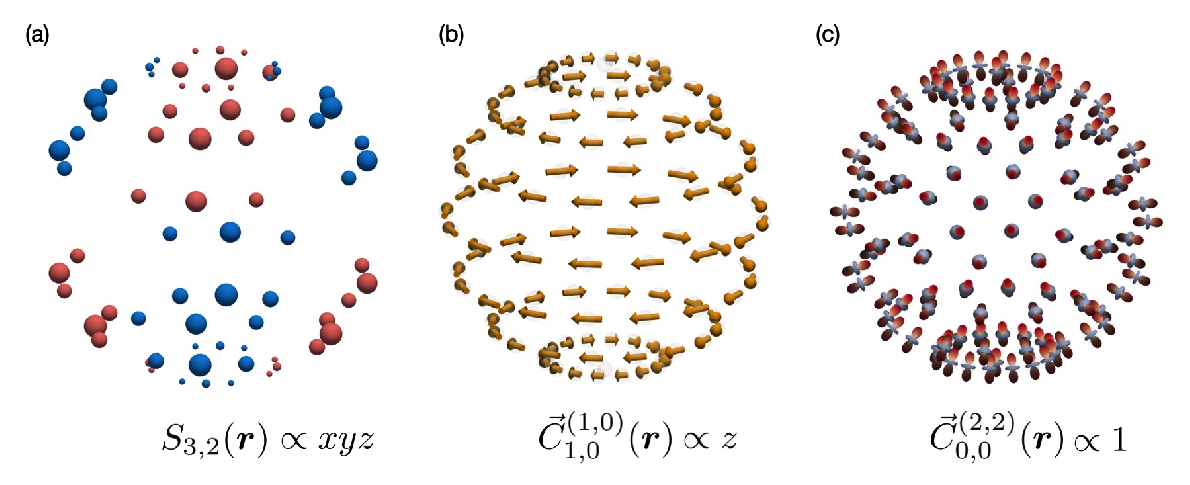
\includegraphics[width=14cm]{fig/m_sh.eps}
  \caption{方域調和関数 (a) $(s,k)=(0,0)$, (b) $(s,k)=(1,0)$, (a) $(s,k)=(2,2)$。}
\label{fig:msh}
\end{figure}

図\ref{fig:msh}に方域調和関数の例を示す。

内部自由度$\vec{q}_{s,n}$または$\vec{g}_{s,n}$の基底として実数を用いるほうが扱いやすいので、方域表示を採用する。
$\vec{q}_{s,\gamma}$ ($s=1,2,3,4$)の定義と$\vec{q}_{s,n}$との関係は、表\ref{tbl:tesbasis}のとおりである。

\begin{table}[t!]
\caption{極性内部自由度の基底。orbital/Wannier90は軌道名。
軸性内部自由度の場合は、{\tt Q}$\to${\tt G}とする。
\label{tbl:tesbasis}}
\begin{center}
\begin{tabular}{cccll} \hline\hline
$s$ & $\gamma$ & name & orbital & Wannier90 \\ \hline
0 & $c(0,0)$ & {\tt Q0} ($q_{0}$) & {\tt s} \\ \hline
1 & $c(1,1)$ & {\tt Qx} ($q_{x}$) & {\tt px} \\
  & $s(1,1)$ & {\tt Qy} ($q_{y}$) & {\tt py} \\
  & $c(1,0)$ & {\tt Qz} ($q_{z}$) & {\tt pz} \\
\hline
2 & $c(2,2)$ & {\tt Qv} ($q_{v}$) & {\tt dv} & {\tt dx2-y2} \\
  & $s(2,2)$ & {\tt Qxy} ($q_{xy}$) & {\tt dxy} \\
  & $c(2,1)$ & {\tt Qxz} ($q_{xz}$) & {\tt dxz} \\
  & $s(2,1)$ & {\tt Qyz} ($q_{yz}$) & {\tt dyz} \\
  & $c(2,0)$ & {\tt Qu} ($q_{u}$) &  {\tt du} & {\tt dz2} \\
\hline
3 & $c(3,3)$ & {\tt Q2} ($q_{2}$) & {\tt f2} & {\tt fx(x2-3y2)} \\
  & $s(3,3)$ & {\tt Q1} ($q_{1}$) & {\tt f1} & {\tt fy(3x2-y2)} \\
  & $c(3,2)$ & {\tt Qbz} ($q_{bz}$) & {\tt fbz} & {\tt fz(x2-y2)} \\
  & $s(3,2)$ & {\tt Q3} ($q_{3}$) & {\tt f3} & {\tt fxyz} \\
  & $c(3,1)$ & {\tt Q3x} ($q_{3x}$) & {\tt f3x} & {\tt fxz2} \\
  & $s(3,1)$ & {\tt Q3y} ($q_{3y}$) & {\tt f3y} & {\tt fyz2} \\
  & $c(3,0)$ & {\tt Qaz} ($q_{az}$) & {\tt faz} & {\tt fz3} \\
\hline\hline
\end{tabular}
\end{center}
\end{table}


\section{原子多極子基底}

\subsection{行列の基底}

\begin{table}[t!]
\begin{center}
\small
\caption{原子多極子基底の軌道基底と基底の順序(球対称)。}
\label{tbl:orbbasis}
\begin{tabular}{cl} \hline\hline
$L$ & basis $(M,\sigma)$ \\ \hline
0 (s) & $\ket{0,\uparrow}$, $\ket{0,\downarrow}$ \\
1 (p) & $\ket{1,\uparrow}$, $\ket{1,\downarrow}$, $\ket{0,\uparrow}$, $\ket{0,\downarrow}$, $\ket{-1,\uparrow}$, $\ket{-1,\downarrow}$ \\
2 (d) & $\ket{2,\uparrow}$, $\ket{2,\downarrow}$, $\ket{1,\uparrow}$, $\ket{1,\downarrow}$, $\ket{0,\uparrow}$, $\ket{0,\downarrow}$, $\ket{-1,\uparrow}$, $\ket{-1,\downarrow}$, $\ket{-2,\uparrow}$, $\ket{-2,\downarrow}$ \\
3 (f) & $\ket{3,\uparrow}$, $\ket{3,\downarrow}$, $\ket{2,\uparrow}$, $\ket{2,\downarrow}$, $\ket{1,\uparrow}$, $\ket{1,\downarrow}$, $\ket{0,\uparrow}$, $\ket{0,\downarrow}$, $\ket{-1,\uparrow}$, $\ket{-1,\downarrow}$, $\ket{-2,\uparrow}$, $\ket{-2,\downarrow}$, $\ket{-3,\uparrow}$, $\ket{-3,\downarrow}$ \\ \hline
$L$ & basis $(J,M)$ \\ \hline
0 (s) & $\ket{\frac{1}{2},\frac{1}{2}}$, $\ket{\frac{1}{2},-\frac{1}{2}}$ \\
1 (p) & $\ket{\frac{1}{2},\frac{1}{2}}$, $\ket{\frac{1}{2},-\frac{1}{2}}$;\quad $\ket{\frac{3}{2},\frac{3}{2}}$, $\ket{\frac{3}{2},\frac{1}{2}}$, $\ket{\frac{3}{2},-\frac{1}{2}}$, $\ket{\frac{3}{2},-\frac{3}{2}}$ \\
2 (d) & $\ket{\frac{3}{2},\frac{3}{2}}$, $\ket{\frac{3}{2},\frac{1}{2}}$, $\ket{\frac{3}{2},-\frac{1}{2}}$, $\ket{\frac{3}{2},-\frac{3}{2}}$;\quad $\ket{\frac{5}{2},\frac{5}{2}}$, $\ket{\frac{5}{2},\frac{3}{2}}$, $\ket{\frac{5}{2},\frac{1}{2}}$, $\ket{\frac{5}{2},-\frac{1}{2}}$, $\ket{\frac{5}{2},-\frac{3}{2}}$, $\ket{\frac{5}{2},-\frac{5}{2}}$ \\
3 (f) & $\ket{\frac{5}{2},\frac{5}{2}}$, $\ket{\frac{5}{2},\frac{3}{2}}$, $\ket{\frac{5}{2},\frac{1}{2}}$, $\ket{\frac{5}{2},-\frac{1}{2}}$, $\ket{\frac{5}{2},-\frac{3}{2}}$, $\ket{\frac{5}{2},-\frac{5}{2}}$; \\
& $\ket{\frac{7}{2},\frac{7}{2}}$, $\ket{\frac{7}{2},\frac{5}{2}}$, $\ket{\frac{7}{2},\frac{3}{2}}$, $\ket{\frac{7}{2},\frac{1}{2}}$, $\ket{\frac{7}{2},-\frac{1}{2}}$, $\ket{\frac{7}{2},-\frac{3}{2}}$, $\ket{\frac{7}{2},-\frac{5}{2}}$, $\ket{\frac{7}{2},-\frac{7}{2}}$ \\
\hline\hline
\end{tabular}
\end{center}
\end{table}

Atomic多極子基底$\hat{X}_{l,m}^{(s,k)}$の定義はJPSJ89, 104704 (2020)に与えられており、この定義に従って$\ket{L,M;\sigma}$軌道基底および$\ket{J,M;L}$軌道基底に対する行列要素をすべて求めることができる。
これらの多極子基底の行列は$(s,p,d,f)\times(s,p,d,f)$ブロックごとに分離することができる。
具体的な軌道基底の順序を表\ref{tbl:orbbasis}にまとめておく。

(\ref{eq:mullinear})と同様に多極子基底の線形結合
\begin{align}
\braket{A|\hat{X}_{l,\gamma}^{(\Gamma,n;s,k)}|B}=\sum_{m}U_{m,\gamma}^{(X,l,\Gamma,n)}\braket{A|\hat{X}_{l,m}^{(s,k)}|B}
\end{align}
により、各点群の多極子基底の行列要素を求める。
$\ket{LM;\sigma}$軌道基底の場合は、実数軌道基底のほうが便利なので、ユニタリー変換$u_{A,r}^{(l,ch)}$ ($ch=$cubic, hexagonal: 表\ref{tbl:uorb})により
\begin{align}
\braket{r|\hat{X}_{l,\gamma}^{(\Gamma,n;s,k)}|s}
=
\sum_{AB}
u_{A,r}^{(l,ch)*}
\braket{A|\hat{X}_{l,\gamma}^{(\Gamma,n;s,k)}|B}
u_{B,s}^{(l,ch)}
=
\braket{r|\hat{u}^{(l,ch)\dagger}
\hat{X}_{l,\gamma}^{(\Gamma,n;s,k)}
\hat{u}^{(l,ch)}|s}
\end{align}
に変換しておく。

スピンレスの多極子基底は$s=k=0$により与えられ、その行列は$\ket{LM;\uparrow}$と$\ket{LM;\downarrow}$のブロックごとに分離し、行列要素は等しい。

\begin{table}[ht!]
\begin{center}
\small
\caption{立方晶/六方晶系の軌道基底と基底の順序。六方晶系の$(yz,-zx)$, $(x^{2}-y^{2},-xy)$のみ、負符号を外すために成分の順序を入れ替えた。}
\label{tbl:uorb}
\begin{tabular}{cl} \hline\hline
$L$ & basis (cubic) \\ \hline
0 (s) & {\tt s} \\ \hline
1 (p) & {\tt px}, {\tt py}, {\tt pz} \\ \hline
2 (d) & {\tt du}, {\tt dv}, {\tt dyz}, {\tt dxz}, {\tt dxy} \\ \hline
3 (f) & {\tt f3}, {\tt fax}, {\tt fay}, {\tt faz}, {\tt fbx}, {\tt fby}, {\tt fbz} \\
\hline\hline
\end{tabular}
\begin{tabular}{cl} \hline\hline
$L$ & basis (hexagonal) \\ \hline
0 (s) & {\tt s} \\ \hline
1 (p) & {\tt px}, {\tt py}, {\tt pz} \\ \hline
2 (d) & {\tt du}, {\tt dxz}, {\tt dyz}, {\tt dxy}, {\tt dv} \\ \hline
3 (f) & {\tt faz}, {\tt f1}, {\tt f2}, {\tt f3x}, {\tt f3y}, {\tt f3}, {\tt fbz} \\
\hline\hline
\end{tabular}
\end{center}
\end{table}

\subsection{正規直交性と完全性}

$\alpha=(X,l,\gamma,\Gamma,n,s,k)$の多極子基底の行列はブラケット表示では$(X_{\alpha})_{m_{1},m_{2}}=\braket{m_{1},m_{2}|\alpha}$である。
多極子基底はhermite行列なので、$\braket{m_{1},m_{2}|\alpha}=\braket{m_{2},m_{2}|\alpha}^{*}$が成り立つ。
$(m_{1},m_{2})$を通し番号$i$で表せば、$(X_{\alpha})_{i}=\braket{i|\alpha}=v_{i,\alpha}$と書ける。

正規直交性は
\begin{align}
\delta_{\alpha\beta}={\rm Tr}(X_{\alpha}^{\dagger }X_{\beta})
=\sum_{\alpha}(X_{\alpha})_{m_{1},m_{2}}^{*}(X_{\beta})_{m_{1},m_{2}}^{}=\sum_{i}\braket{\alpha|i}\braket{i|\beta}=(v^{\dagger}v)_{\alpha\beta}
\label{eq:orthonormal}
\end{align}
完全性は
\begin{align}
\delta_{ij}
=\sum_{m_{1}m_{2}}(X_{\alpha})_{m_{1},m_{2}}(X_{\alpha})_{m_{3},m_{4}}^{*}=\sum_{\alpha}\braket{i|\alpha}\braket{\alpha|j}
=(vv^{\dagger})_{ij}
\label{eq:completeness}
\end{align}
と表現される。

多極子基底の行列は$(L_{1},L_{2})$のブロックに分解されるので、$L_{1}=L_{2}$の場合は、各ブロックで上記の正規直交性と完全性が成り立つ\footnote{ブロック$(L_{1},L_{2})$やタイプ$X$が異なる場合は直交するので、正規直交化はブロックおよびタイプごとに行えばよい。}。

$L_{1}\ne L_{2}$のときは、独立な多極子基底は$N=2(2L_{1}+1)(2L_{2}+1)$個ある。
多極子基底を上三角成分を纏めたものを$u_{i,\alpha}$ ($u$は$N/2\times N$行列)とすると、上三角成分は$v_{i\alpha}=u_{i\alpha}$, 下三角成分は$v_{i\alpha}=u_{i\alpha}^{*}$である。
(\ref{eq:orthonormal})の$i$の和は上三角成分か下三角成分を指すから、$(v^{\dagger}v)_{\alpha\beta}=2{\rm Re}(u^{\dagger}u)_{\alpha\beta}$となる。
また、(\ref{eq:completeness})の$i,j$は上(下)三角と下(上)三角の成分間の場合は$(vv^{\dagger})_{ij}=(u u^{t})_{ij}$ ($(u u^{t})_{ij}^{*}$)、上三角(下三角)の成分間では$(vv^{\dagger})_{ij}=(uu^{\dagger})_{ij}$ ($(uu^{\dagger})_{ij}^{*}$)である。
$u^{\dagger}u$, $uu^{\dagger(t)}$は$N\times N$行列および$N/2\times N/2$行列である。
したがって、正規直交性と完全性はそれぞれ
\begin{align}
&
\delta_{\alpha\beta}=2{\rm Re}[(u^{\dagger}u)]_{\alpha\beta}
\cr&
0
=(uu^{t})_{ij},
\quad
1=(uu^{\dagger})_{ij}
\end{align}
となる。

\subsection{与えられた制限軌道空間での使用}

実際に原子多極子を用いる際は、軌道を制限することになる。
$L\Gamma\gamma$表示で用意されている軌道の一部を使用する場合は、対応する行列要素を抜き出した後、$(L_{1},L_{2})$ブロックごとに再直交化を行えばよい。
より一般の軌道を用いる場合は、用意されている軌道表示$\gamma$から用いたい軌道表示$\alpha$への変換行列$T_{\gamma,\alpha}=\braket{\gamma|\alpha}$を与え、これを用いて変換した後、$(L_{1},L_{2})$ブロックごとに再直交化を行う。

正規直交化の際、直交化前の基底を$(Q/G/T/M,s,k,l,\Gamma,n)$の順に並べておくとよい\footnote{多極子タイプ, $s$, $k$ごとに低ランクの基底を優先するため。}。

\end{document}
